%
% Assignment Template
% Last modified 9/11/2024 by Ziyong Wang

\documentclass[11pt]{article}
\usepackage[left=0.7in,right=0.7in,top=1in,bottom=0.7in]{geometry}
\usepackage{fancyhdr} % for header
\usepackage{graphicx} % for figures
\usepackage{amsmath}  % for extended math markup
\usepackage{amssymb}
\usepackage{inconsolata}
\usepackage{enumitem}
\usepackage{float}
\usepackage[bookmarks=false]{hyperref} % for URL embedding
\usepackage[noend]{algpseudocode} % for pseudocode
\usepackage[plain]{algorithm} % float environment for algorithms

%%%%%%%%%%%%%%%%%%%%%%%%%%%%%%%%%%%%%%%%%%%%%%%%%%%%%%%%%%%%%%%%%%%%%%

\newcommand{\Course}{FIN 550E}
\newcommand{\GroupNumber}{27}
\newcommand{\ProjectNumber}{1}

%%%%%%%%%%%%%%%%%%%%%%%%%%%%%%%%%%%%%%%%%%%%%%%%%%%%%%%%%%%%%%%%%%%%%%%%

% create header and footer for every page
\pagestyle{fancy}
\fancyhf{}
\lhead{\textbf{\Course}}
\chead{\textbf{Group \GroupNumber}}
\rhead{\textbf{Empirical Project \ProjectNumber}}
\cfoot{\thepage}

% preferred pseudocode style
\algrenewcommand{\algorithmicprocedure}{}
\algrenewcommand{\algorithmicthen}{}

% ``do { ... } while (cond)''
\algdef{SE}[DOWHILE]{Do}{doWhile}{\algorithmicdo}[1]{\algorithmicwhile\ #1}%

% ``for (x in y ... z)''
\newcommand{\ForRange}[3]{\For{#1 \textbf{in} #2 \ \ldots \ #3}}

% these are common math formatting commands that aren't defined by default
\newcommand{\union}{\cup}
\newcommand{\isect}{\cap}
\newcommand{\ceil}[1]{\ensuremath \left\lceil #1 \right\rceil}
\newcommand{\floor}[1]{\ensuremath \left\lfloor #1 \right\rfloor}

%%%%%%%%%%%%%%%%%%%%%%%%%%%%%%%%%%%%%%%%%%%%%%%%%%%%%%%%%%%%%%%%%%%%%%

\begin{document}

% text goes here!

\section{Part 1: data preparation}

\begin{enumerate}
\renewcommand{\labelenumi}{(\theenumi)}
    \item \, \\
    \begin{table}[H]
        \centering
        \begin{tabular}{lccc}
        \hline
         & \textbf{s} & \textbf{netwin1} & \textbf{netwin2} \\
        \hline
        \textbf{mean} & -0.034295 & 0.000546 & 0.008731 \\
        \textbf{std} & 6.910801 & 0.085145 & 0.340307 \\
        \textbf{min} & -1790.209 & -0.890778 & -1.071007 \\
        \textbf{10th percentile} & -0.005455 & -0.083904 & -0.316339 \\
        \textbf{25th percentile} & -0.000437 & -0.033229 & -0.152914 \\
        \textbf{median} & 0.000331 & 0.000182 & -0.012081 \\
        \textbf{75th percentile} & 0.001659 & 0.034908 & 0.128584 \\
        \textbf{90th percentile} & 0.004961 & 0.084568 & 0.313767 \\
        \textbf{max} & 7.432727 & 1.588795 & 22.972540 \\
        \hline
        \end{tabular}
        \caption{Summary Statistics for Earnings Surprises (s), Market-Adjusted Returns for Windows [0,1] (netwin1) and [3,75] (netwin2)}
    \end{table}

    \item
        
\end{enumerate}

\section{Part 2: short-run response}

\begin{enumerate}
\setcounter{enumi}{2}
\renewcommand{\labelenumi}{(\theenumi)}
    \item \, \\
    
    \begin{figure}[H] 
        \centering
        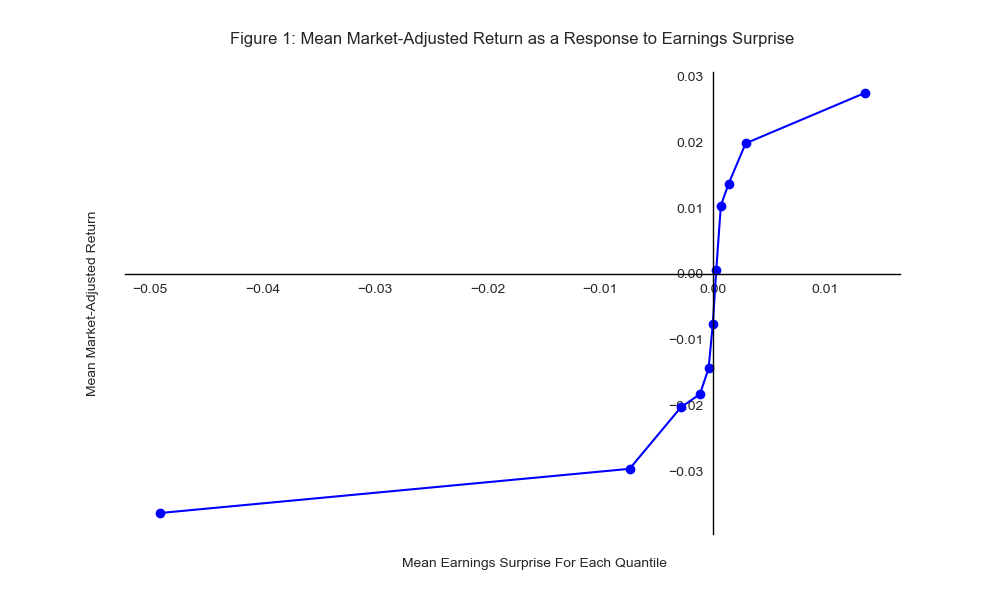
\includegraphics[width=.8\textwidth]{fig1.png}
    \end{figure}

    \begin{figure}[H] 
        \centering
        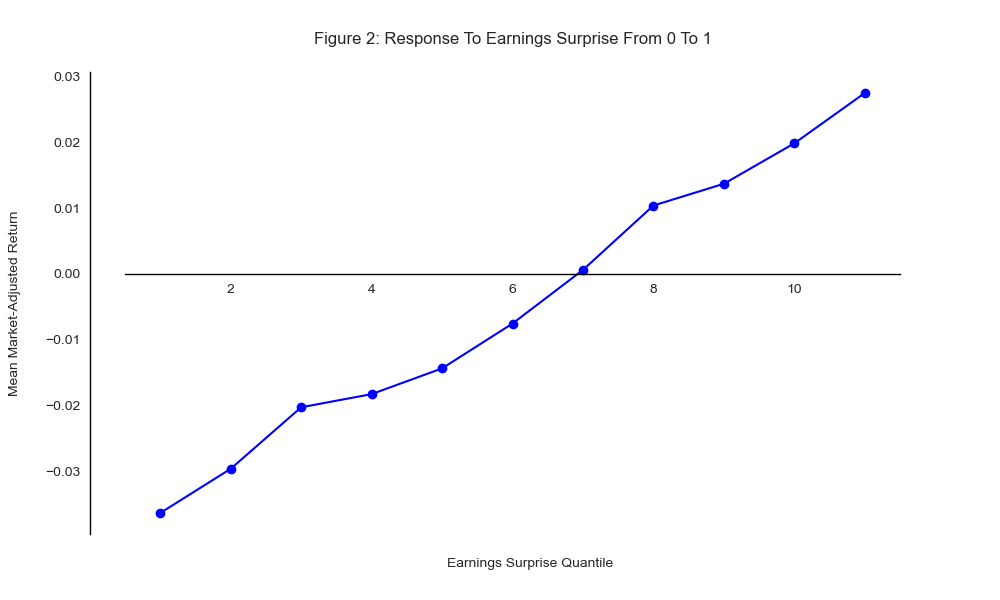
\includegraphics[width=.8\textwidth]{fig2.png}
    \end{figure}
    
    \item
    
    \item

\end{enumerate}

\section{Part 3: Post-earnings announcement drift}

\begin{enumerate}
\setcounter{enumi}{5}
\renewcommand{\labelenumi}{(\theenumi)}
    \item \, \\
    \begin{figure}[H] 
        \centering
        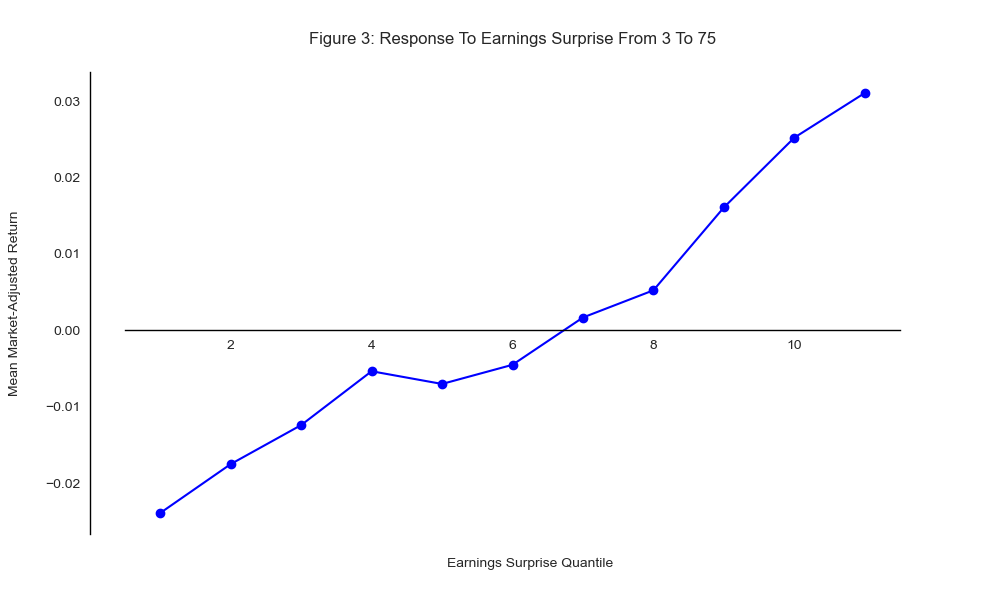
\includegraphics[width=.8\textwidth]{fig3.png}
    \end{figure}
    
    \item
    
    \item

\end{enumerate}

\section{Part 4: Inattention and distractions}

\begin{enumerate}
\setcounter{enumi}{8}
\renewcommand{\labelenumi}{(\theenumi)}
    \item 

\end{enumerate}

\section{Part 5: Open-ended}

\begin{enumerate}
\setcounter{enumi}{9}
\renewcommand{\labelenumi}{(\theenumi)}
    \item 

    \item

\end{enumerate}

\section{Appendix}
\begin{figure}[H] 
    \centering
    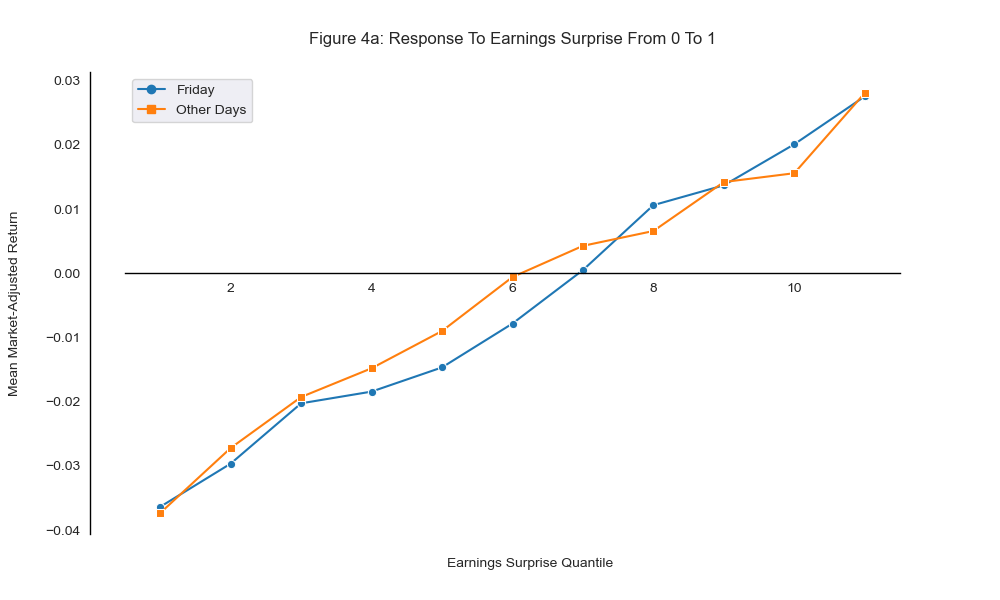
\includegraphics[width=.8\textwidth]{fig4a.png}
\end{figure}

\begin{figure}[H] 
    \centering
    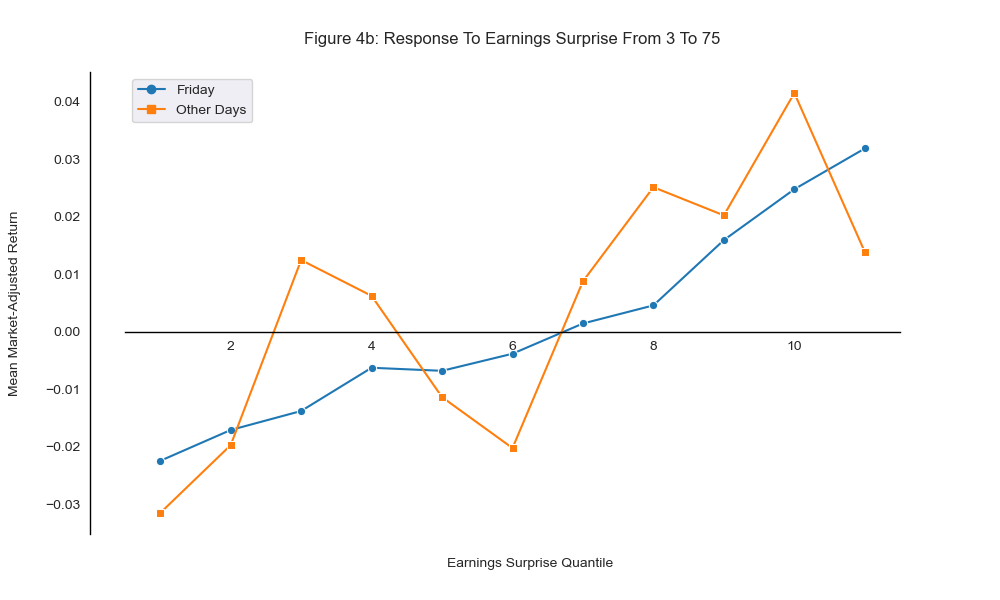
\includegraphics[width=.8\textwidth]{fig4b.png}
\end{figure}

\begin{figure}[H] 
    \centering
    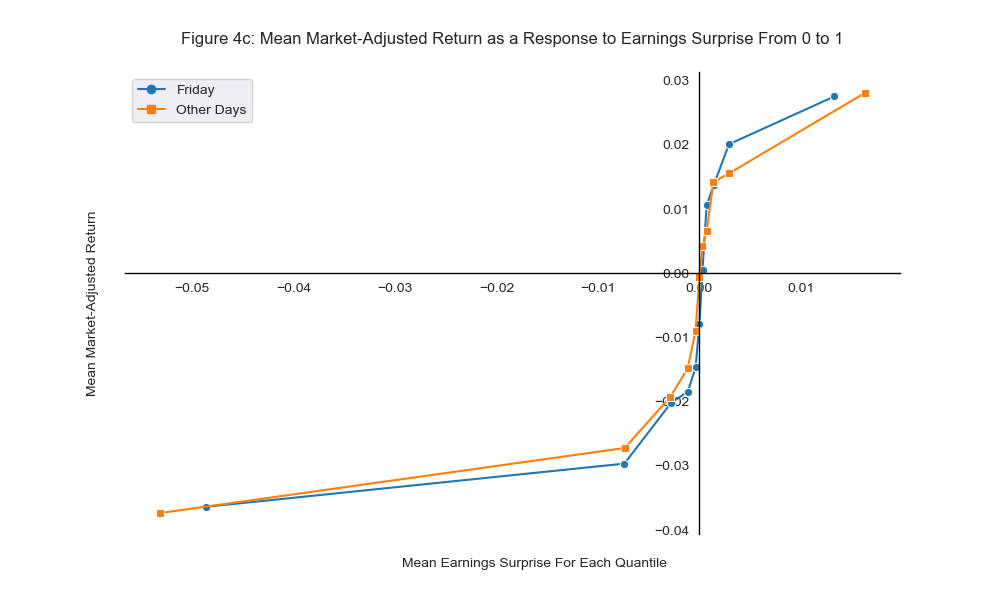
\includegraphics[width=.8\textwidth]{fig4c.png}
\end{figure}

\begin{figure}[H] 
    \centering
    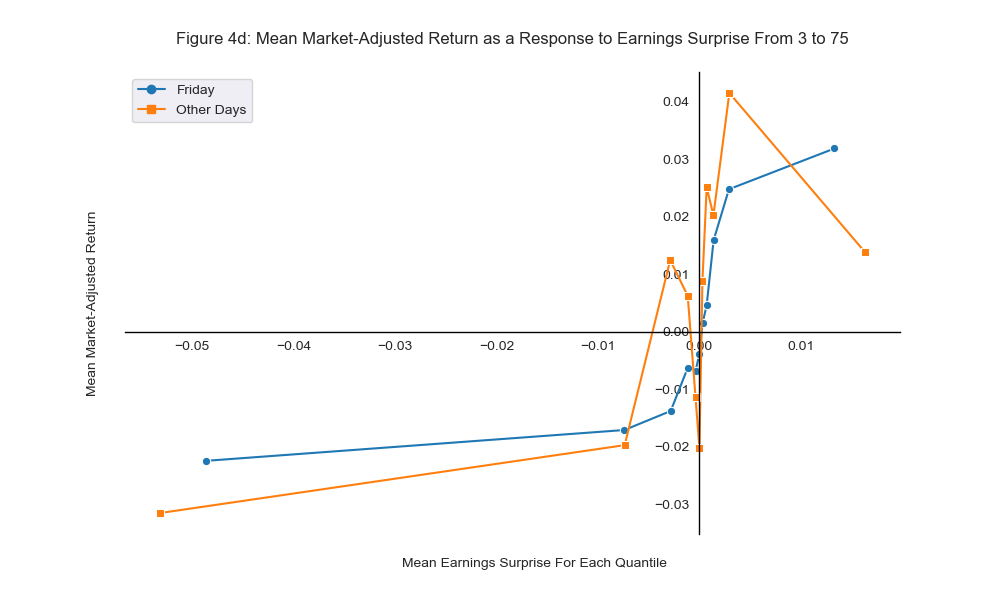
\includegraphics[width=.8\textwidth]{fig4d.png}
\end{figure}

\end{document}
